%\documentclass[letterpaper]{article}
%\usepackage{beamerarticle}
%\documentclass{beamer}
\documentclass[handout]{beamer}

\usepackage{genchem}
\graphicspath{{../../Figures/}}
\usepackage[thicklines,makeroom]{cancel}

\renewcommand{\CancelColor}{\color{red}}

\title[Chapter 7.01-05]{Reactions in Aqueous Solution}
\author{CHEM111}

\begin{document}

\frame{\titlepage}

\begin{frame}{Some Ways That Chemical Reactions Occur}
	\begin{itemize}
		\item Precipitation
		\item Acid-Base Neutralization
		\item Oxidation-Reduction (Redox)
	\end{itemize}
\end{frame}

\begin{frame}[allowframebreaks]{Oxidation-Reduction (Redox) Reactions}
	Processes in which one or more electrons are transferred between
	reaction partners (atoms, molecules, or ions)

	\begin{center}
		\ce{Mg(s) + 2HCl(aq) -> MgCl2(aq) + H2(g)}
	\end{center}

	\framebreak

	\begin{itemize}
		\item \textbf{Oxidation}
			\begin{itemize}
				\item The \emph{loss} of one or more electrons
					by a substance, whether element,
					compound, or ion.
			\end{itemize}
		\item \textbf{Reduction}
			\begin{itemize}
				\item The \emph{gain} of one or more electrons
					by a substance, whether element,
					compound, or ion.
			\end{itemize}
	\end{itemize}

	\begin{center}
		\includegraphics[scale=0.3]{07_Pg249_UnFigure_1.jpg}
	\end{center}

	\framebreak

	The rusting of iron is an \textbf{oxidation} reaction:

	\begin{center}
		\ce{4Fe(s) + 3O2(g) -> 2Fe2O3(s)}
	\end{center}

	The manufacture of iron is a \textbf{reduction} reaction:

	\begin{center}
		\ce{2Fe2O3(s) + 3C(s) -> 4Fe(s) + 3CO2(g)}
	\end{center}
\end{frame}

\begin{frame}[allowframebreaks=0.9]{Assigning Oxidation Numbers}
	\begin{enumerate}
		\item An atom in its elemental state has an oxidation
			number of 0.

			\begin{center}
				\includegraphics[height=4em]{07_Pg249_UnFigure_2.jpg}
			\end{center}
		\item An atom in a monatomic ion has an oxidation
			number identical to its charge.

			\begin{center}
				\includegraphics[height=4em]{07_Pg249_UnFigure_3.jpg}
			\end{center}
		\item An atom in a polyatomic ion or in a molecular
			compound usually has the same oxidation number it would
			have if it were a monatomic ion.

			\begin{center}
				\includegraphics[height=5em]{07_Pg249_UnFigure_4.jpg}
			\end{center}

			\textbf{Recall:} nonmetals are more ``anionlike'' and
			metals are more ``cationlike''

			\framebreak

			\begin{enumerate}
				\item Hydrogen can be either +1 or -1

					\begin{center}
						\includegraphics[height=3em]{07_Pg250_UnFigure_2.jpg}
					\end{center}

				\item Oxygen \emph{usually} has an oxidation
					number of -2
				
					\begin{center}
						\includegraphics[height=3em]{07_Pg250_UnFigure_3.jpg}
					\end{center}

				\item Halogens \emph{usually} have an oxidation
					number of -1

					\begin{center}
						\includegraphics[height=3em]{07_Pg250_UnFigure_4.jpg}
					\end{center}
			\end{enumerate}

			\framebreak

		\item The sum of the oxidation numbers is 0 for a neutral
			compound and is equal to the net charge for a polyatomic
			ion.
			\bigskip

			\begin{center}
				\includegraphics[height=3em]{07_Pg250_UnFigure_5.jpg}

				\bigskip

				\includegraphics[height=3em]{07_Pg250_UnFigure_6.jpg}
			\end{center}
	\end{enumerate}

	\framebreak

	Assign oxidation numbers to each atom in the following substances:

	\begin{itemize}
		\item \ce{HClO4}
		\item \ce{ClO3-}
		\item \ce{K2Cr2O7}
		\item \ce{MnO4-}
		\item \ce{H2O2}
	\end{itemize}
\end{frame}

\begin{frame}[allowframebreaks]{Identifying Redox Reactions}
	\begin{itemize}
		\item A redox reaction involves a change in \textbf{oxidation
			number}

			\begin{center}
				\includegraphics[height=6em]{07_Pg251_UnFigure_3.jpg}
			\end{center}
		\item For every \textbf{oxidation}, there must be a
			\textbf{reduction}

			\begin{center}
				\includegraphics[height=6em]{07_Pg252_UnFigure_1.jpg}
			\end{center}
	\end{itemize}

	\framebreak

	\textbf{\color{blue} Reduction Agent}
	\begin{itemize}
		\item Causes reduction
		\item Loses one or more electrons
		\item Undergoes oxidation
		\item Oxidation number of atom increases
	\end{itemize}

	\bigskip

	\textbf{\color{red} Oxidizing Agent}
	\begin{itemize}
		\item Causes oxidation
		\item Gains one or more electrons
		\item Undergoes reduction
		\item Oxidation number of atom decreases
	\end{itemize}

	\framebreak

	Identify the oxidizing agent and the reducing agent in each reaction
	\textbf{if} it is a redox reaction:

	\begin{itemize}
		\item \ce{P4(s) + 5O2(g) -> P4O10(s)}
		\item \ce{Co(s) + Cl2(g) -> CoCl2(s)}
		\item \ce{ZnO(s) + C(s) -> Zn(s) + CO(g)}
		\item \ce{AgNO3(aq) + NaBr(aq) -> AgBr(s) + NaNO3(aq)}
		\item \ce{8Fe(s) + S8(s) -> 8FeS(s)}
	\end{itemize}

\end{frame}

\begin{frame}[allowframebreaks]{The Activity Series of the Elements}
	\begin{itemize}
		\item We have previously seen single-displacement reactions,
			where one element replaces another in a compound

			\begin{center}
				\ce{Fe(s) + Cu^{2+}(aq) -> Fe^{2+}(aq) + Cu(s)}

				\medskip

				\ce{Mg(s) + 2H+(aq) -> Mg^{2+}(aq) + H2(g)}
			\end{center}

		\item Do the reverse reactions occur \emph{spontaneously?}

			\begin{center}
				\ce{Fe(s) + Cu^{2+}(aq) <-[{?}] Fe^{2+}(aq) + Cu(s)}

				\medskip

				\ce{Mg(s) + 2H+(aq) <-[{?}] Mg^{2+}(aq) + H2(g)}
			\end{center}
			\framebreak
		\item The \textbf{activity series} ranks elements in order of
			their reducing ability in aqueous solution

			\begin{center}
				\includegraphics[scale=0.3]{07_05_Table.jpg}
			\end{center}
		\item Elements that are higher up on the table are more likely
			to be \textbf{oxidized}
		\item Elements higher in the activity series will
			\textbf{reduce} the ion of any element lower in the
			activity series

			\begin{center}
				\ce{Cu(s) + 2Ag+(aq) -> Cu^{2+}(aq) + 2Ag(s)}

				\medskip

				\ce{Au(s) + 3Ag+(aq) \xcancel{\ce{->}}
				Au^{3+}(aq) + Ag(s)} 
				
				\emph{\tiny\color{red} Does
				not occur}
			\end{center}
		\item Note that most easily oxidized metals are located to the
			left of the periodic table and therefore have
			\textbf{low ionization energies}
	\end{itemize}

	\framebreak

	Will the following reactions occur?

	\begin{itemize}
		\item \ce{2H+(aq) + Pt(s) -> H2(g) + Pt^{2+}(aq)}
		\item \ce{Ca^{2+}(aq) + Mg(s) -> Ca(s) + Mg^{2+}(aq)}
		\item \ce{2Cr(s) + 3Sn^{2+} -> 2Cr^{3+} + 3Sn(s)}
		\item \ce{2Li(s) + Co^{2+}(aq) -> 2Li+(aq) + Co(s)}
	\end{itemize}
\end{frame}

\begin{frame}{Balancing Redox Reactions}
	\begin{itemize}
		\item Recognize that every redox reaction must have both an
			oxidation and a reduction reaction
		\item The oxidation and reduction reactions can be split into
			two parts -- \textbf{half-reactions}
		\item We will find which element is being oxidized and which is
			being reduced and balance each half-reaction
			\textbf{independently}
	\end{itemize}
\end{frame}

\begin{frame}{Balancing Redox Reactions: Acidic Solution}
	Balance the following net ionic equation in \textbf{acidic} solution:

	\begin{center}
		\ce{I-(aq) + Cr2O7^{2-}(aq) -> Cr^{3+}(aq) + IO3-(aq)}
	\end{center}

	\begin{enumerate}[<+->]
		\item Write the two unbalanced half-reactions
			\mode<article>{
				\begin{center}
				\begin{tabular}{r@{ \ce{->} }l}
					\ce{Cr2O7^{2-}(aq)} & \ce{Cr^{3+}(aq)}
					\\
					\ce{I-(aq)} & \ce{IO3-(aq)}
				\end{tabular}
			\end{center}}
		\item Balance both half-reactions for all atoms
			except O and H
			\mode<article>{\begin{center}
				\begin{tabular}{r@{ \ce{->} }l}
					\ce{Cr2O7^{2-}(aq)} & \ce{2Cr^{3+}(aq)}
					\\
					\ce{I-(aq)} & \ce{IO3-(aq)}
				\end{tabular}
			\end{center}}
		\item Balance each half-reaction for O by adding
			\ce{H2O}
			\mode<article>{\begin{center}
				\begin{tabular}{r@{ \ce{->} }l}
					\ce{Cr2O7^{2-}(aq)} & \ce{2Cr^{3+}(aq) +
					7H2O(l)}
					\\
					\ce{3H2O(l) + I-(aq)} & \ce{IO3-(aq)}
				\end{tabular}
			\end{center}}
		\item Balance each half-reaction for H by adding \ce{H+}
			\mode<article>{\begin{center}
				\begin{tabular}{r@{ \ce{->} }l}
					\ce{14H+(aq) + Cr2O7^{2-}(aq)} &
					\ce{2Cr^{3+}(aq) + 7H2O(l)}
					\\
					\ce{3H2O(l) + I-(aq)} & \ce{IO3-(aq) +
					6H+(aq)}
				\end{tabular}
			\end{center}}
		\item Balance each half-reactions for charge by adding electrons
			to the side with greater positive charge
			\mode<article>{\begin{center}
				\begin{tabular}{r@{ \ce{->} }l}
					\ce{6e- + 14H+(aq) + Cr2O7^{2-}(aq)} &
					\ce{2Cr^{3+}(aq) + 7H2O(l)}
					\\
					\ce{3H2O(l) + I-(aq)} & \ce{IO3-(aq) +
					6H+(aq) + 6e-}
				\end{tabular}
			\end{center}}
		\item Multiply each half-reaction by a factor to make the
			electron count the same in both half-reactions
			\mode<article>{\begin{center}
				\begin{tabular}{r@{ \ce{->} }l L}
					\ce{6e- + 14H+(aq) + Cr2O7^{2-}(aq)} &
					\ce{2Cr^{3+}(aq) + 7H2O(l)} & \times 1
					\\
					\ce{3H2O(l) + I-(aq)} & \ce{IO3-(aq) +
					6H+(aq) + 6e-} & \times 1
				\end{tabular}
			\end{center}}
		\item Add the two balanced half-reactions together
			\mode<article>{\begin{center}
				\begin{tabular}{r@{ \ce{->} }l}
					\ce{6e- + 14H+(aq) + Cr2O7^{2-}(aq)} &
					\ce{2Cr^{3+}(aq) + 7H2O(l)}
					\\
					\ce{3H2O(l) + I-(aq)} & \ce{IO3-(aq) +
					6H+(aq) + 6e-} \\
					\midrule
					\multicolumn{2}{l}{\ce{6e- + 14H+(aq) +
					Cr2O7^{2-}(aq) + 3H2O(l) + I-(aq)}} \\
					\multicolumn{2}{r}{\ce{-> 2Cr^{3+}(aq) +
					7H2O(l) + IO3-(aq) + 6H+(aq) + 6e-}}
				\end{tabular}
			\end{center}}
		\item Cancel species that appear on both sides of the equation
			\mode<article>{\begin{center}
				\begin{tabular}{r@{ \ce{->} }l}
					\multicolumn{2}{l}{\ce{\cancel{\ce{6e-}}
					+ \cancelto{8}{14}H+(aq) +
					Cr2O7^{2-}(aq) + \cancel{\ce{3H2O(l)}} +
					I-(aq)}} \\
					\multicolumn{2}{r}{\ce{-> 2Cr^{3+}(aq) +
					\cancelto{4}{7}H2O(l) + IO3-(aq) +
					\cancel{\ce{6H+(aq)}} +
					\cancel{\ce{6e-}}}} \\
					\midrule
					\multicolumn{2}{l}{\ce{8H+(aq) +
					Cr2O7^{2-}(aq) + I-(aq)}} \\
					\multicolumn{2}{r}{\ce{-> 2Cr^{3+}(aq) +
					4H2O(l) + IO3-(aq) }}
				\end{tabular}
			\end{center}}
	\end{enumerate}
\end{frame}

\begin{frame}{Balancing Redox Reactions: Basic Solution}
	Balance the following net ionic equation in \textbf{basic} solution:

	\begin{center}
		\ce{MnO4-(aq) + Br-(aq) -> MnO2(s) + BrO3-(aq)}
	\end{center}

	\begin{enumerate}
		\item Write the two unbalanced half-reactions
			\mode<article>{
				\begin{center}
				\begin{tabular}{r@{ \ce{->} }l}
					\ce{Br-(aq)} & \ce{BrO3-(aq)}
					\\
					\ce{MnO4-(aq)} & \ce{MnO2(s)}
				\end{tabular}
			\end{center}}
		\item Balance both half-reactions for all atoms
			except O and H
			\mode<article>{\begin{center}
				\begin{tabular}{r@{ \ce{->} }l}
					\ce{Br-(aq)} & \ce{BrO3-(aq)}
					\\
					\ce{MnO4-(aq)} & \ce{MnO2(s)}
				\end{tabular}
			\end{center}}
		\item Balance each half-reaction for O by adding
			\ce{H2O}
			\mode<article>{\begin{center}
				\begin{tabular}{r@{ \ce{->} }l}
					\ce{3H2O(l) + Br-(aq)} & \ce{BrO3-(aq)}
					\\
					\ce{MnO4-(aq)} & \ce{MnO2(s) + 2H2O(l)}
				\end{tabular}
			\end{center}}
		\item Balance each half-reaction for H by adding \ce{H+}
			\mode<article>{\begin{center}
				\begin{tabular}{r@{ \ce{->} }l}
					\ce{3H2O(l) + Br-(aq)} & \ce{BrO3-(aq) +
					6H+(aq)}
					\\
					\ce{4H+(aq) + MnO4-(aq)} & \ce{MnO2(s) +
					2H2O(l)}
				\end{tabular}
			\end{center}}
		\item Balance each half-reactions for charge by adding electrons
			to the side with greater positive charge
			\mode<article>{\begin{center}
				\begin{tabular}{r@{ \ce{->} }l}
					\ce{3H2O(l) + Br-(aq)} & \ce{BrO3-(aq) +
					6H+(aq) + 6e-}
					\\
					\ce{3e- + 4H+(aq) + MnO4-(aq)} &
					\ce{MnO2(s) + 2H2O(l)}
				\end{tabular}
			\end{center}}
		\item Multiply each half-reaction by a factor to make the
			electron count the same in both half-reactions
			\mode<article>{\begin{center}
				\begin{tabular}{r@{ \ce{->} }l L}
					\ce{3H2O(l) + Br-(aq)} & \ce{BrO3-(aq) +
					6H+(aq) + 6e-}
					\\
					\ce{3e- + 4H+(aq) + MnO4-(aq)} &
					\ce{MnO2(s) + 2H2O(l)} & \times 2
				\end{tabular}
			\end{center}}
		\item Add the two balanced half-reactions together
			\mode<article>{
				\begin{center}
				\begin{tabular}{r@{ \ce{->} }l}
					\ce{3H2O(l) + Br-(aq)} & \ce{BrO3-(aq) +
					6H+(aq) + 6e-}
					\\
					\ce{6e- + 8H+(aq) + 2MnO4-(aq)} &
					\ce{2MnO2(s) + 4H2O(l)} \\
					\midrule
					\multicolumn{2}{l}{\ce{3H2O(l) + Br-(aq)
					+ 6e- + 8H+(aq) + 2MnO4-(aq)}} \\
					\multicolumn{2}{r}{\ce{-> BrO3-(aq) +
					6H+(aq) + 6e- + 2MnO2(s) + 4H2O(l)}}
				\end{tabular}
			\end{center}}
		\item Cancel species that appear on both sides of the equation
			\mode<article>{\begin{center}
				\begin{tabular}{r@{ \ce{->} }l}
					\multicolumn{2}{l}{\ce{
						\cancel{\ce{3H2O(l)}}
					+ Br-(aq) + \cancel{\ce{6e-}} +
					\cancelto{2}{8}H+(aq) + 2MnO4-(aq)}} \\
					\multicolumn{2}{r}{\ce{-> BrO3-(aq) +
					\cancel{\ce{6H+(aq)}} +
					\cancel{\ce{6e-}} + 2MnO2(s) +
					\cancelto{1}{4}H2O(l)}}
					\\
					\midrule
					\multicolumn{2}{l}{\ce{ Br-(aq) +
					2H+(aq) + 2MnO4-(aq)}} \\
					\multicolumn{2}{r}{\ce{-> BrO3-(aq) +
					2MnO2(s) + H2O(l)}}
				\end{tabular}
			\end{center}}
		\item<2> \bfseries ``Neutralize'' excess \ce{H+} by adding
			\ce{OH-} and cancel \ce{H2O}
			\mode<article>{\begin{center}
				\begin{tabular}{r@{ \ce{->} }l}
					\multicolumn{2}{l}{\ce{2OH-(aq) +
					Br-(aq) + 2H+(aq) + 2MnO4-(aq)}} \\
					\multicolumn{2}{r}{\ce{-> BrO3-(aq) +
					2MnO2(s) + H2O(l) + 2OH-(aq)}}
				\end{tabular}
			\end{center}
			
			Recall \ce{H+(aq) + OH-(aq) -> H2O(l)}

			\begin{center}
				\begin{tabular}{r@{ \ce{->} }l}
					\multicolumn{2}{l}{\ce{
						Br-(aq) + \cancelto{1}{2}H2O(l)
						+ 2MnO4-(aq)}} \\
						\multicolumn{2}{r}{\ce{->
						BrO3-(aq) + 2MnO2(s) +
						\cancel{\ce{H2O(l)}} +
						2OH-(aq)}} \\
						\midrule
					\multicolumn{2}{l}{\ce{
						Br-(aq) + H2O(l)
						+ 2MnO4-(aq)}} \\
						\multicolumn{2}{r}{\ce{->
						BrO3-(aq) + 2MnO2(s) +
						2OH-(aq)}}
				\end{tabular}
			\end{center}
			}
	\end{enumerate}
\end{frame}

\begin{frame}{Balancing Redox Practice}
	Balance the following equations in \textbf{acidic} solution:
	\begin{itemize}
		\item \ce{CuCl2(aq) + Al(s) -> AlCl3(aq) + Cu(s)}
		\item \ce{Cr^{3+}(aq) + Zn(s) -> Cr(s) + Zn^{2+}(aq)}
	\end{itemize}

	\bigskip

	Balance the following equations in \textbf{basic} solution:
	\begin{itemize}
		\item \ce{FeI3(aq) + Mg(s) -> Fe(s) + MgI2(aq)}
		\item \ce{H2(g) + Ag+(aq) -> Ag(s) + H+(aq)}
	\end{itemize}
\end{frame}

\begin{frame}[allowframebreaks]{Redox Titrations}
	\begin{itemize}
		\item \textbf{Titration}
			\begin{itemize}
				\item A procedure for determining the
					concentration of a solution by allowing
					a carefully measured volume to react
					with a solution of another substance
					(the standard solution) whose
					concentration is known.
			\end{itemize}

			\bigskip
		\item Redox (like all) titrations must demonstrate 100\% yield
		\item A change must be observable at the endpoint
	\end{itemize}
		
	\framebreak
	Aqueous \ce{KMnO4} reacts with oxalic acid (\ce{H2C2O4}) and is
	accompanied by a color change:

		{\mhchemoptions{mathfontcommand=\mathsf}
		\footnotesize
		\begin{align*}
			\ce{5H2C2O4(aq) + &2MnO4-(aq) + 6H+(aq) \\
			-> &10CO2(g) + 2Mn^{2+}(aq) + 8H2O(l)}
		\end{align*}}

		\begin{center}
			\includegraphics[scale=0.6]{07_06_Figure.jpg}
		\end{center}
\end{frame}

\begin{frame}{Redox Stoichiometry}
	A solution is prepared with \SI{0.2585}{\gram} oxalic acid
	(\ce{H2C2O4}). \SI{22.35}{\milli\liter} of an unknown solution of
	potassium permanganate \ce{KMnO4} is needed to titrate the solution.
	What is the concentration of the potassium permanganate solution?

	{\mhchemoptions{mathfontcommand=\mathsf}
		\footnotesize
		\begin{align*}
			\ce{5H2C2O4(aq) + &2MnO4-(aq) + 6H+(aq) \\
			-> &10CO2(g) + 2Mn^{2+}(aq) + 8H2O(l)}
		\end{align*}}

	\begin{center}
		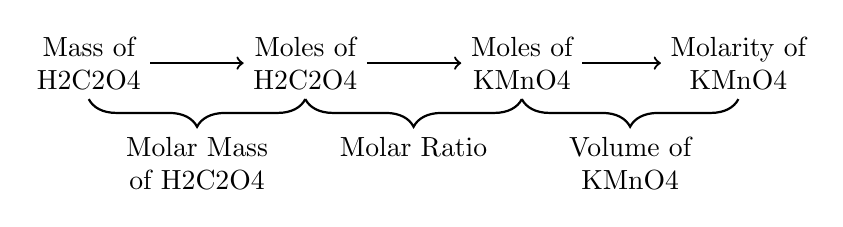
\begin{tikzpicture}
			\node[align=center](Ag) at (0,0){Mass of \\
			\ce{H2C2O4}};
			\node[align=center](Am) at (2.75,0){Moles of \\
			\ce{H2C2O4}} ;
			\node[align=center](Bm) at (5.5,0){Moles of \\
			\ce{KMnO4}} ;
			\node[align=center](Bg) at (8.25,0){Molarity of \\
			KMnO4} ;
			\draw[thick,->] (Ag.east) -- (Am.west);
			\draw[thick,->] (Am.east) -- (Bm.west);
			\draw[thick,->] (Bm.east) -- (Bg.west);
			\draw[thick,decorate,decoration={
				brace,
				mirror,
				amplitude=10pt}] (Ag.south) -- (Am.south)
				node[below,midway,align=center,yshift=-10pt]
				{Molar Mass \\ of \ce{H2C2O4}};
			\draw[thick,decorate,decoration={
				brace,
				mirror,
				amplitude=10pt}] (Am.south) -- (Bm.south)
				node[below,midway,align=center,yshift=-10pt]
				{Molar Ratio};
			\draw[thick,decorate,decoration={
				brace,
				mirror,
				amplitude=10pt}] (Bm.south) -- (Bg.south)
				node[below,midway,align=center,yshift=-10pt]
				{Volume of \\ \ce{KMnO4}};
		\end{tikzpicture}
	\end{center}

	\mode<article>{
		\begin{tabular}{r L@{ = }S}
			Moles \ce{H2C2O4}: & \SIce{0.2585}{\gram}{H2C2O4} \times
			\dfrac{\SI{1}{\mole}}{\SI{90.04}{\gram}} &
			\SIce{0.002871}{\mole}{H2C2O4} \\
			Moles \ce{KMnO4}: & \SIce{0.002871}{\mole}{H2C2O4}
			\times
			\dfrac{\SIce{2}{\mole}{KMnO4}}{\SIce{5}{\mole}{H2C2O4}}
			& \SIce{0.001148}{\mole}{KMnO4} \\
			Concentration: & \dfrac{\SIce{0.001148}{\mole}{KMnO4}}
			{\SI{22.35}{\milli\liter}} \times
			\dfrac{\SI{1000}{\milli\liter}}{\SI{1}{\liter}} &
			\SIce{0.05136}{\Molar}{KMnO4}
		\end{tabular}}
\end{frame}

\begin{frame}{Some Applications of Redox Reactions}
	\begin{itemize}
		\item Combustion

			\begin{center}
				\ce{CH4(g) + 2O2(g) -> CO2(g) + 2H2O(l)}
			\end{center}

		\item Bleaching
		\item Batteries

			\begin{center}
				\ce{LiC6 + CoO2 <=> C6 + LiCoO2}
			\end{center}

		\item Metallurgy

			\begin{center}
				\ce{ZnO(s) + C(s) -> Zn(s) + CO(g)}
			\end{center}

		\item Corrosion
			
			\begin{center}
				\ce{4Fe(s) + 3O2(g) ->[H2O] 2Fe2O3.H2O(s)}
			\end{center}

		\item Respiration
			
			\begin{center}
				\ce{C6H12O6 + 6O2 -> 6CO2 + 6H2O +
				\text{energy}}
			\end{center}
	\end{itemize}
\end{frame}

\end{document}
